\documentclass{bfh}
\usepackage[numbers]{natbib}

\title{Bachelor Thesis}
\subtitle{An Android Client for Bitmessage}
\author{Christian Basler}
\advisor{Kai Brünnler}
\expert{Daniel Voisard}
\date{\today}

\begin{document}
  \maketitle

  \tableofcontents

  \listoffigures

  \newpage
  \section*{Abstract}

  Even if we use encryption, we reveal a lot about ourselves in the metadata we produce. Bitmessage prevents this by distributing a message in a way that it's not possible to find out which was the intended recipient.
  
  This thesis aims to develop an Android client for the Bitmessage protocol.

  \newpage

  \section{Introduction}

  \subsection{What is Metadata?}

  While encryption technology like PGP or S/MIME provides a secure way to protect content from prying eyes, ever since the revelations of whistleblower Edward Snowdens we learned that metadata --- most notably information about who communicates with whom --- is equally interesting and much easier to analyse.\cite{guardian:metadata}

  \subsection{How Can We Hide Metadata?}

  With e-mail, all metadata is plain text, even for encrypted messages. We might be able to encrypt the connection to the e-mail provider, and they might or might not encrypt their connections to other providers. We can only hope that both our and the recipient's e-mail provider are both trustworthy and competent. Can we really expect that from something we get for free?

  With Bitmessage we send a message to a sufficiently large number of participants, with the intended recipient among them. Content is encrypted such that only the person in possesion of the private key can decrypt it. All participants try to do this in order to find their messages.

  \subsection{What is Bitmessage}
  
  Bitmessage is a peer to peer protocol building a mesh network among the participating clients. Every client tries to maintain multiple connections and has a full copy of every current object.
  
  Objects are encrypted using a public key. Every client tries to decrypt each object using its private keys, processing the ones where it succeeds.
  
  A bit advantage of Bitmessage is its inherent key management. The address contains a hash of the public key, and retrieving said key is part of the protocol.

  (TODO)\newpage

  \subsection{Current state -- why is it bad?}
  Until recently there was no mobile client for Bitmessage, and the client that turned up since is very wasteful to the devices resources, draining the battery in little time. The alternative is to use an e-mail relay server, but this means to give up the private key to this server and end-to-end encryption is much more difficult to achieve. Therefore this might not be a viable option, especially if you can't run your own server.

  \subsection{How should it be?}
  We need mobile Bitmessage clients that allows the user to choose their levels of convenience, privacy and resource hunger. There will always be trade-offs between needed traffic, battery use and privacy, and for each user the answer might look slightly different.

  \subsection{Why is it hard to do?}
  Bitmessage is very wasteful with resources by design. All messages are being sent to and stored on all nodes, and to protect the network proof of work (POW) is required for all objects that are distributed. The protocol wasn't developed with mobile users in mind, and while smartphones are getting increasingly powerful, there is at least the issue of battery use to watch out for, and most users have limited traffic on their data plan.

  \subsection{Why me, and how do I intend to do it?}
  I have seven years of experience developing Java applications, and was programming Android apps from the moment I had my ``Android Dev Phone 1''. As I developed Jabit, a Java implementation of the Bitmessage client, as my last project, I also have great knowledge about the Bitmessage protocol.

  There are a few optimisations that I intend to do:
  \begin{itemize}
    \item Connect to only one reliable node instead of eight random nodes. This should reduce battery usage, but yields some risk if the node is compromised. Also, the node must forward all messages to all connected mobile clients instead of the default eight random nodes.
    \item Don't save objects we can't decrypt. We can solely save their hashes, but this means we're using the network without supporting it. This also might be an attack vector.
    \item Only connect to the network if we're on Wi-Fi and charging. This means of course that we'll only receive messages when we're connected with a Wi-Fi and charging.
  \end{itemize}
  Of course every option has its own drawbacks, so they will be configurable. As for the POW: Jabit highly optimises its calculation, which might be enough for modern smartphones.

  Further optimisations might introduce a server component that might do
  \begin{itemize}
    \item POW
    \item Request public keys, requiring us to give up some anonymity towards the server.
    \item Inform the client about new messages sent to its addresses. This would mean to give up our anonymity towards the server in the best case (which isn't supported by the protocol yet), towards the whole network (which is somewhat supported), or give up the private key to the server (which is just a big NOPE).
  \end{itemize}

  \subsection{Jabit Architecture}
  Jabit follows the Ports and Adapters architecture. There is a domain module which contains all the data types and most parts of the protocol implementation, and provides several ports, to which adapters can be attached. Adapters include the data repositories, network code and, more recently, cryptography (see BC vs. SC).

  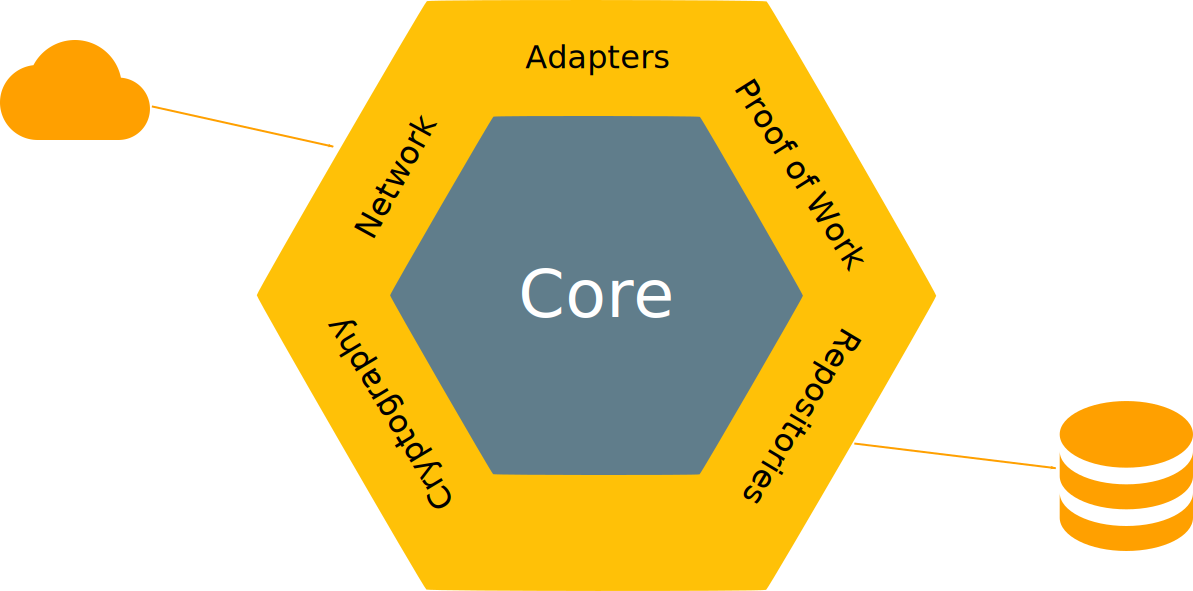
\includegraphics[width=\textwidth]{images/ports_and_adapters.pdf}
  
  \section{Naive Implementation}
  
  The naive implementation attempts to use the Jabit Bitmessage library as it is, with as little mobile optimisations as possible.

  \subsection{Unexpected Problems}
  Most problems can be summarised as this: Android builds on the Java language, but not on the Java platform.
  
  \subsubsection{Bouncy Castle vs. Spongy Castle}
  Jabit heavily relies on the Bouncy Castle library for all things encryption. Unfortunately, Android ships with a broken version of Bouncy Castle. Even worse, when building an Android app the toolchain just discards any Bouncy Castle dependencies in favor of the built-in, broken version.

  Some people recognised this problem, and built a fork of Bouncy Castle, called Spongy Castle. It basically just replaces “Bouncy” with “Spongy” wherever necessary, so it doesn’t get discarded during the build process. This works fine and is quite easily done. Unfortunately, this doesn’t work on the Desktop.

  The Oracle JVM requires Security Providers to be signed, which is done for Bouncy Castle builds, but not so for the Spongy derivation. As forking Jabit wasn’t an option, the whole Security part had to be refactored in an exchangeable module, and implemented twice, in both a bouncy and a spongy manifestation.

  \subsubsection{JDBC}
  Android has its own API to access the included SQLite database. While it’s a nice, easy to use API, the Android team didn’t deem it necessary to support JDBC, which is the Java standard API to connect to databases.

  There is an open source project attempting to implement a JDBC driver for Android’s SQLite database called SQLDroid,\footnote{\url{https://github.com/SQLDroid/SQLDroid}} which looked very promising. Unfortunately, it lacks essential features, such as returning the automatically generated key of an inserted row. Even worse, it doesn't have the courtesy of throwing a NotImplementedException for missing features, instead it just does nothing and returns null where a result is required.

  Unfortunately, discovering SQLDroid was unfit for the job took more time than reimplementing all repositories using the Android database API. As they were already implemented as adapters, no change was necessary on the Jabit library.

  \subsection{Expected Problems}
  Those problems were to be expected and need to be fixed in part II.

  \subsubsection{Proof of Work}
  Although modern smartphones tend to have faster processors than cheap personal computers, proof of work for sending a public key takes around 15 minutes on a device with four cores at 2.5 GHz. Even worse, during this time it uses so much power that the device discharges even when connected to a power supply.

  \section{Optimisations}
  \subsection{Sync Adapters}
  Android provides an API that can vastly reduce battery usage for apps that regularly update data over the internet. The system triggers synchronisation, so it can optimise its sleep modes. Imagine otherwise, 15 apps synchronising every 15 minutes, one after the other. The device would never sleep.

  Although it's not intended, synchronisation can be done within the Bitmessage protocol without any modifications. What is needed is a trusted node that's always available and therefore best run on a proper server. On successful connection all new messages are being exchanged, so we just need to connect, wait until new messages were exchanged, and then disconnect.

  As Jabit is a Java library, it was trivial to create a server application using Spring Boot and Jabit. It turned out though that it's necessary to limit the number of connections in a Bitmessage server, therefore connections are now being severed after 12 hours or when a limit of 100 connections is reached.

  \bibliographystyle{plain}
  \bibliography{bibliography}

\end{document}